\documentclass[../thesis]{subfiles}

\begin{document}
	\subsection{Results}
	\label{subsec:mic:native:results}

	\begin{figure}[htp]
		\begin{center}
			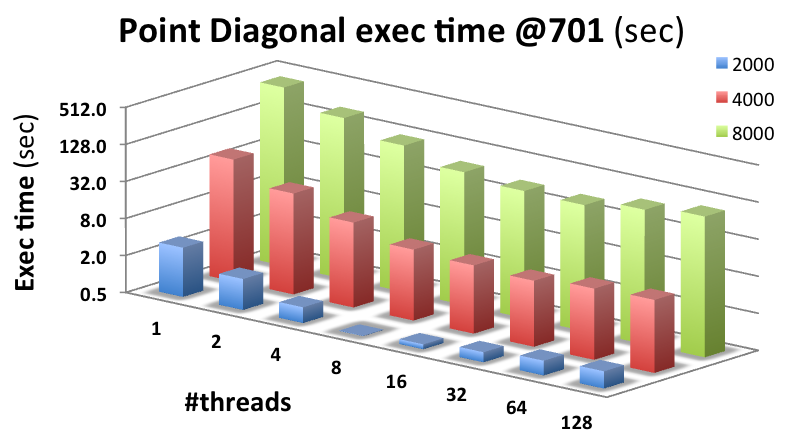
\includegraphics[width=0.9\textwidth]{assets/images/mic/point-diagonal.png}
		\end{center}
		\caption{Execution times for point method and diagonal strategy in the \intel\xeonphi}
		\label{fig:mic:point:diagonal:times}
	\end{figure}

	\begin{figure}[htp]
		\begin{center}
			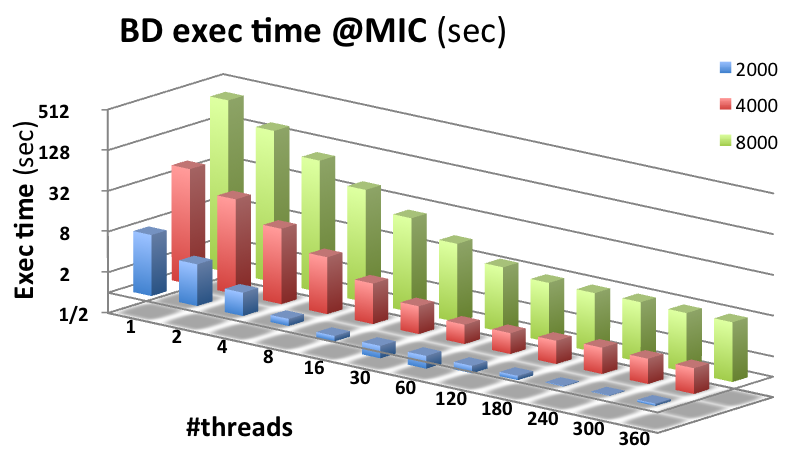
\includegraphics[width=0.9\textwidth]{assets/images/mic/block-diagonal.png}
		\end{center}
		\caption{Execution times for block method and diagonal strategy in the \intel\xeonphi}
		\label{fig:mic:block:diagonal:times}
	\end{figure}

	\Cref{fig:mic:point:diagonal:times,fig:mic:block:diagonal:times} show the obtained execution times using the diagonal strategy for both methods as described in \cref{chp:multicore}. The scalability of the algorithm is near perfect for both, with the execution time being cut almost by half until the number of threads matches the number of cores in the device. After that, the speedup slows down, with the point method reaching its peak performance when using 4 hardware threads per core (full Hyper-Threading) and the block method plateauing at 2 hardware threads per core. The block method performance only leaves this plateau when 8 or more threads per core are used.

	\begin{figure}[htp]
		\begin{center}
			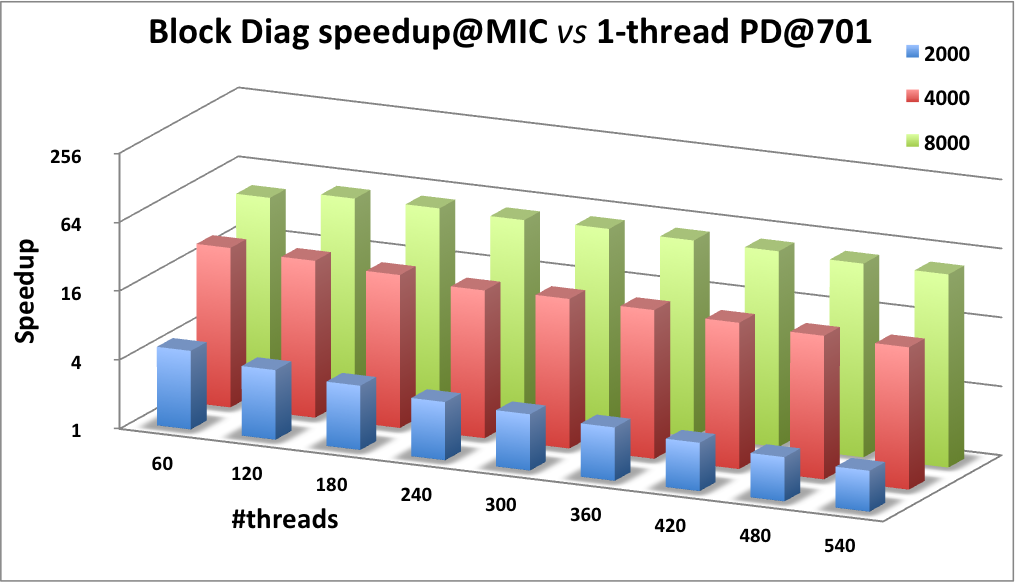
\includegraphics[width=0.9\textwidth]{assets/images/mic/mic-cpu-speedup-accumulated.png}
		\end{center}
		\caption{Accumulated speedup from block-diagonal in the \intel\xeonphi versus point-diagonal in the \cpu}
		\label{fig:mic:mic-cpu:speedup:accumulated}
	\end{figure}

	\begin{figure}[htp]
		\begin{center}
			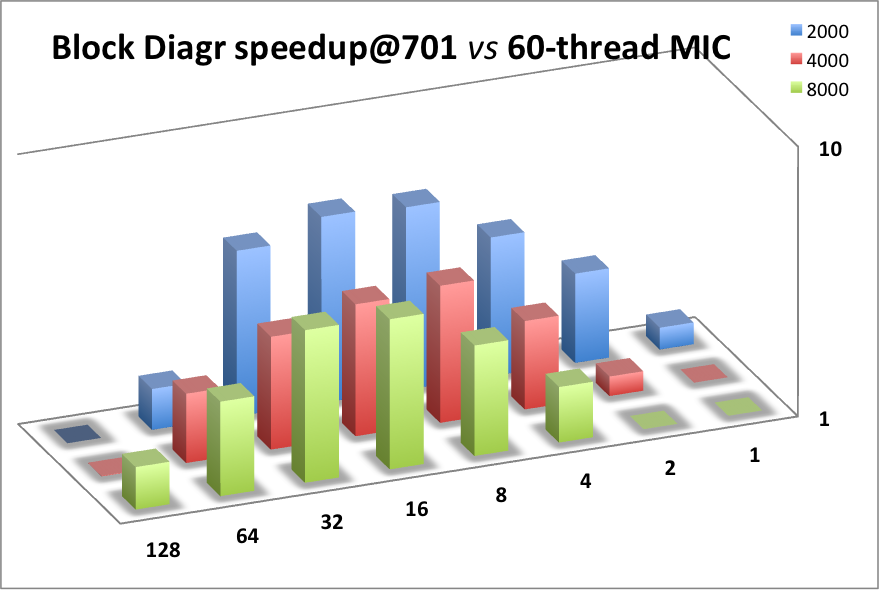
\includegraphics[width=0.9\textwidth]{assets/images/mic/cpu-mic-speedup.png}
		\end{center}
		\caption{Speedup from block-diagonal in the \cpu versus in the \intel\xeonphi (using 60 threads)}
		\label{fig:mic:cpu-mic:speedup}
	\end{figure}

	Although the accumulated speedup of executing the block-diagonal in the \intel\xeonphi, when compared to the point method in the \cpu, is still significant, it does not even reach half of the accumulated speedup achieved in the \cpu. In fact, when comparing the accumulated speedups in both platforms, the best value obtained in the \intel\xeonphi is about three times slower than the best value obtained in the \cpu.
\end{document}
